\pagenumbering{arabic}
%\documentclass[slides]{beamer}
\documentclass[mathserif,10pt]{beamer}
%\documentclass[slides,hyperref={pdfpagelabels=false}]{beamer}
%\documentclass[handout,gray]{beamer}
\usepackage[T1]{fontenc}
\usepackage[utf8]{inputenc}
\usepackage{textcomp}
\usepackage{verbatim}
\usepackage{amsbsy}
\usepackage{multicol}
\usepackage{booktabs} % Make some nice tables
\usepackage{ae,aecompl}

%%%%%%%%%%%% COULEURS %%%%%%%%%%%%%%%%%%%%%%%%%%%

\mode<presentation>
{
  \definecolor{beamerstructure}{RGB}{43,79,112}
  \definecolor{sidebackground}{RGB}{230,242,250}
  \definecolor{CTCC}{RGB}{133,188,228}
  \color{beamerstructure}
  \usetheme{default}
  \usepackage{courier}
  \beamertemplateballitem
\setbeamertemplate{navigation symbols}{}
%\setbeamertemplate{sidebar left}{\thispdfpagelabel{\insertframenumber}}
%\setbeamertemplate{footline}{\quad\insertframenumber}
%\usecolortheme{CTCC}
}
\usebackgroundtemplate{\includegraphics[width=1.02\paperwidth]{../templets/ctcc_general.jpg}}

\title{\\\vspace{1cm} Relativistic effects in chemistry}
%\subtitle{\textcolor{magenta}{My subtitle (if applicable)}}
\author{Stig Rune Jensen}
\institute[CTCC]{\\[-6mm]stig.r.jensen@uit.no\\[6mm]UiT The Arctic University of Norway\\[6mm]
\includegraphics[height=1.5cm]{../templets/uio.pdf}\hspace{1cm} 
\includegraphics[height=1.5cm]{../templets/sff.pdf}\hspace{1cm}
\includegraphics[height=1.5cm]{../templets/uit.pdf}}
\date{Troms\o, March 20th 2014}

\newcommand{\gb}[1]{green!#1!black}
\newcommand{\rb}[1]{red!#1!black}
\newcommand{\bb}[1]{blue!#1!black}
\newcommand{\coleq}{red!60!black}
\newcommand{\du}{\textrm{d}}

\usepackage{multicol}
\newcommand{\mydef}{\stackrel{\text{def}}{\hbox{=}}} 

\begin{document}

\footnotesize
\setlength{\unitlength}{\textwidth}

{
\usebackgroundtemplate{\includegraphics[width=1.02\paperwidth]{../templets/ctcc_forside.jpg}}
\maketitle
}

\begin{frame}
    \frametitle{Outlook}
\end{frame}

\begin{frame}
    \frametitle{Relativistic effects in physics}
    \begin{columns}
    \begin{column}{.50\textwidth}
	\ \\
    \end{column}
    \begin{column}{.50\textwidth}
	\centering
	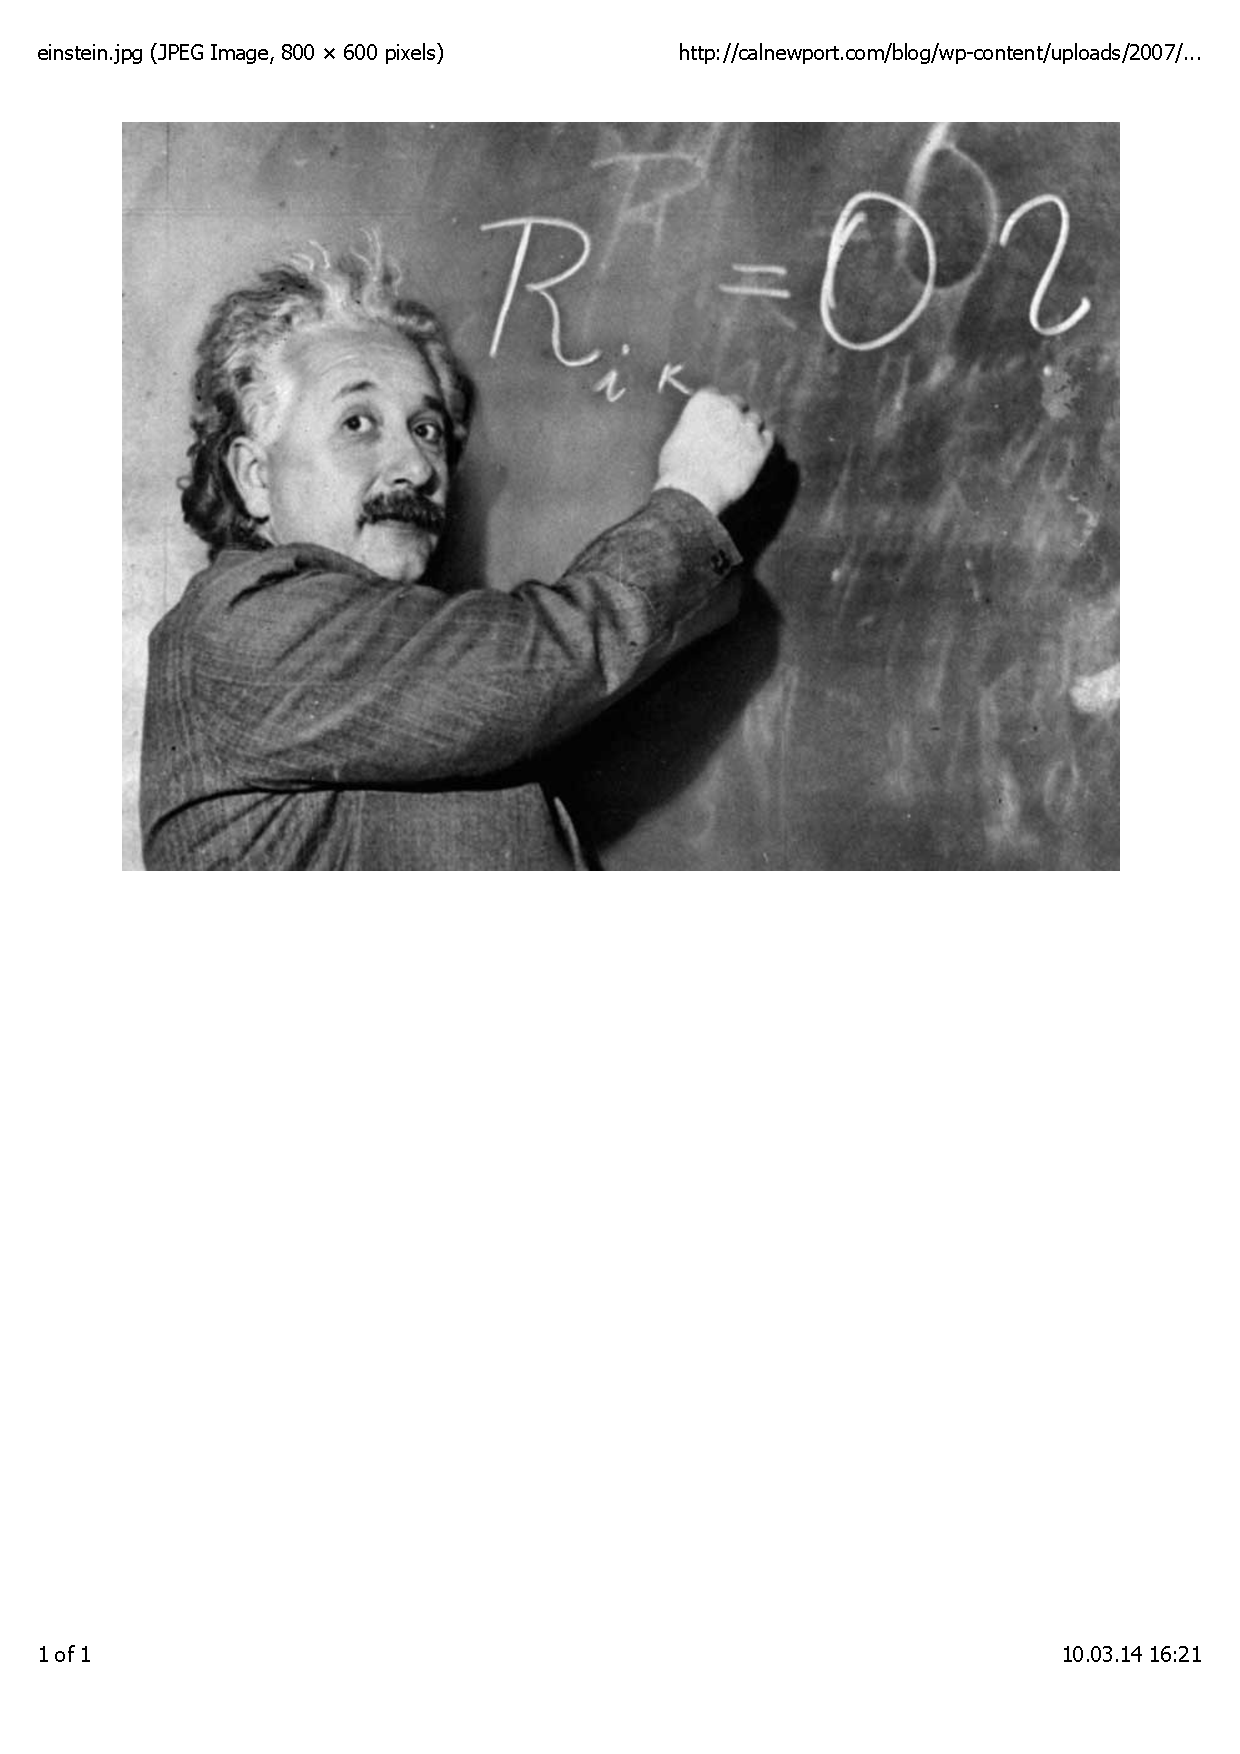
\includegraphics[viewport = 50 450 550 750, clip, scale=0.2]{figures/einstein.pdf}
    \end{column}
    \end{columns}
\end{frame}

\begin{frame}
    \frametitle{Relativistic energy}
    \begin{columns}
    \begin{column}{.50\textwidth}
	\begin{equation}
	    \nonumber
	    E^2 = \boldsymbol{p}^2c^2 + m^2c^4
	\end{equation}
	\ \\
	\ \\
	\begin{equation}
	    \nonumber
	    E = mc^2
	\end{equation}
    \end{column}
    \begin{column}{.50\textwidth}
	\centering
	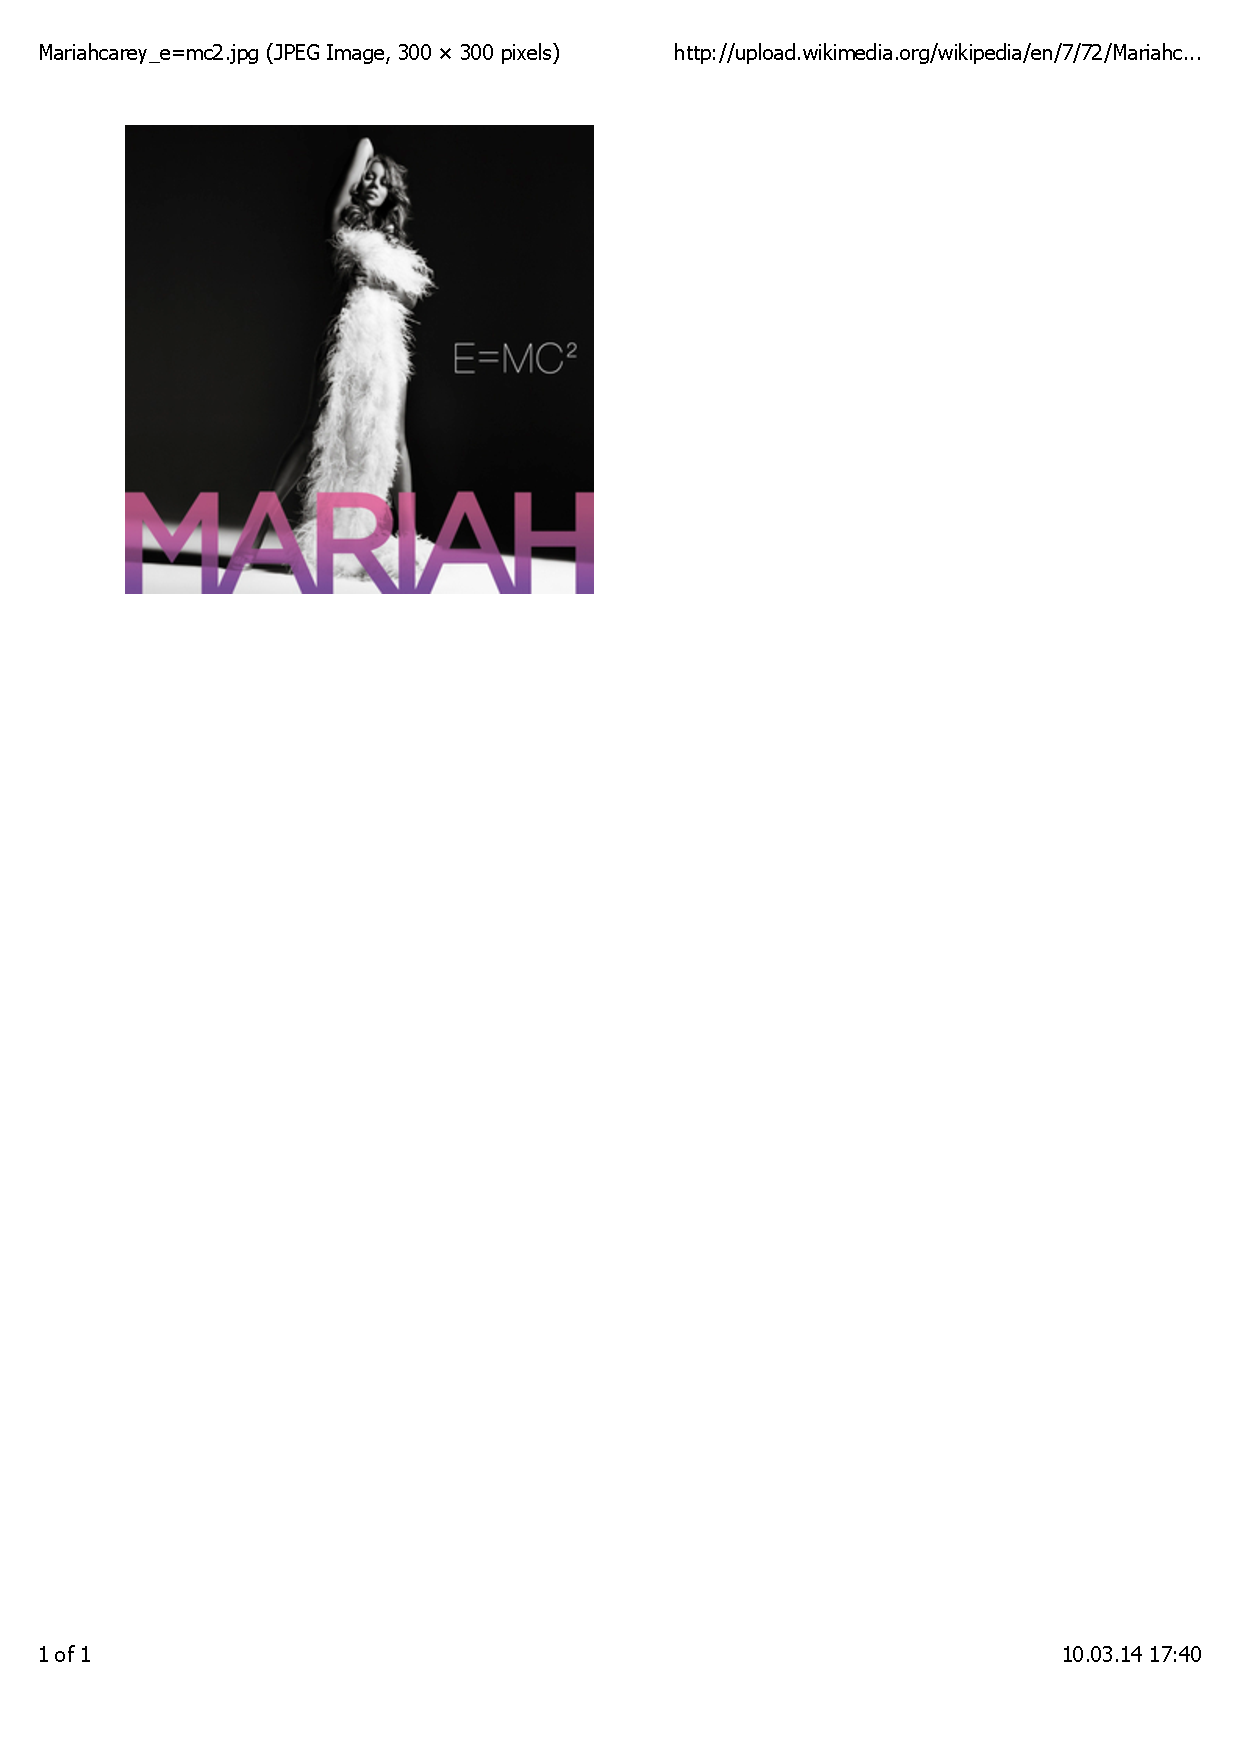
\includegraphics[viewport = 60 560 285 800, clip, scale=0.4]{figures/mariah.pdf}
    \end{column}
    \end{columns}
\end{frame}

\begin{frame}
    \frametitle{Relativistic effects in chemistry}
    \begin{columns}
    \begin{column}{.6\textwidth}
	\centering
	\begin{exampleblock}{\it{\small{''These [relativistic effects] give rise to difficulties 
	    only when high-speed particles are involved, and are therefore of \textcolor{red}{no 
	    importance} in the consideration of atomic and molecular structure and ordinary 
	    chemical reactions\dots''}}}
	    \vskip2mm
	    \hspace*\fill{\tiny--- Paul AM Dirac, 1929}
	\end{exampleblock}
    \end{column}
    \begin{column}{.4\textwidth}
	\centering
	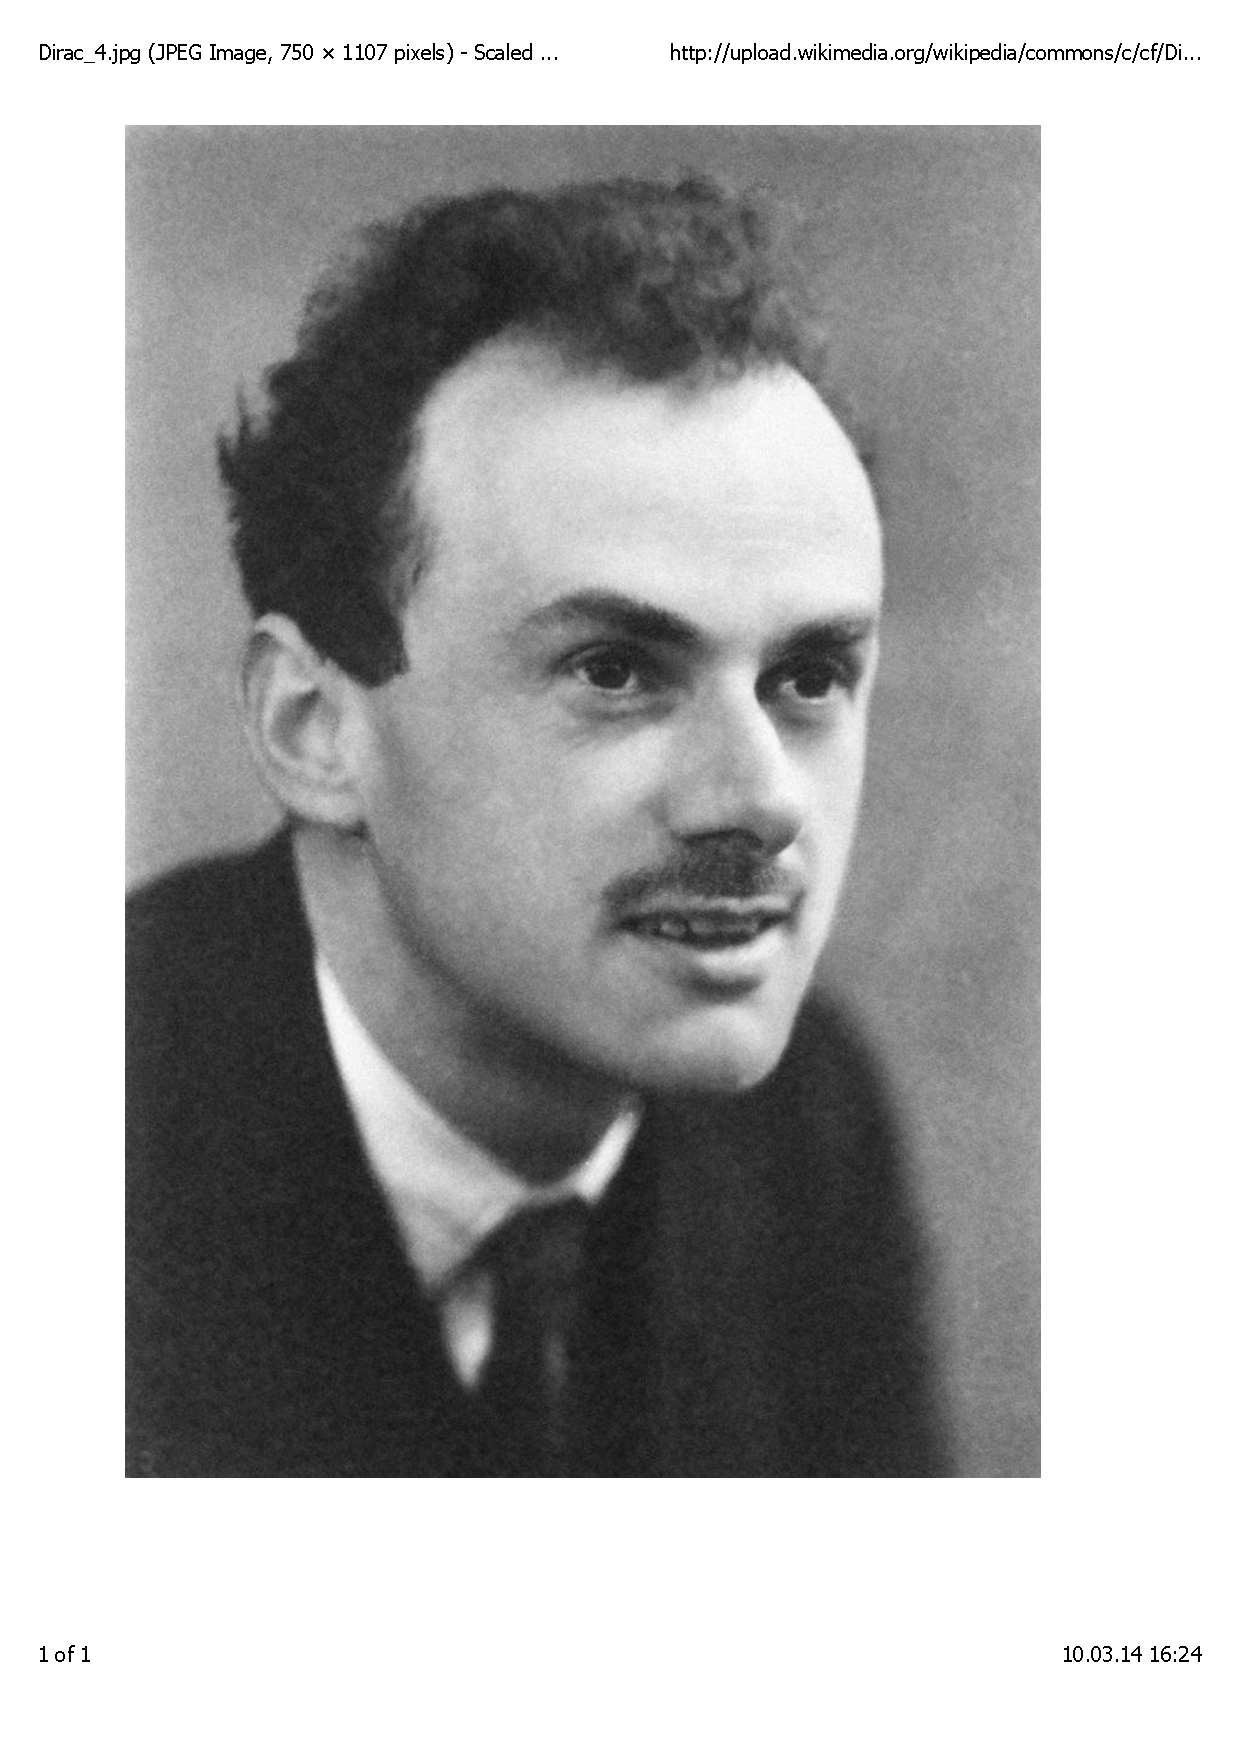
\includegraphics[viewport = 50 200 500 800, clip, scale=0.15]{figures/dirac.pdf}
    \end{column}
    \end{columns}
\end{frame}

\begin{frame}
    \frametitle{The Schr\"{o}dinger equation}
    \begin{columns}
    \begin{column}{.50\textwidth}
	\begin{equation}
	\nonumber
	    \hat{H} \psi = E \psi
	\end{equation}
	\ \\
	\ \\
	\begin{equation}
	\nonumber
	    \hat{H} = \sum_i h(\boldsymbol{r}_i) + \frac{1}{2}\sum_{i,j} g(\boldsymbol{r}_i,\boldsymbol{r}_j)
	\end{equation}
    \end{column}
    \begin{column}{.50\textwidth}
	\centering
	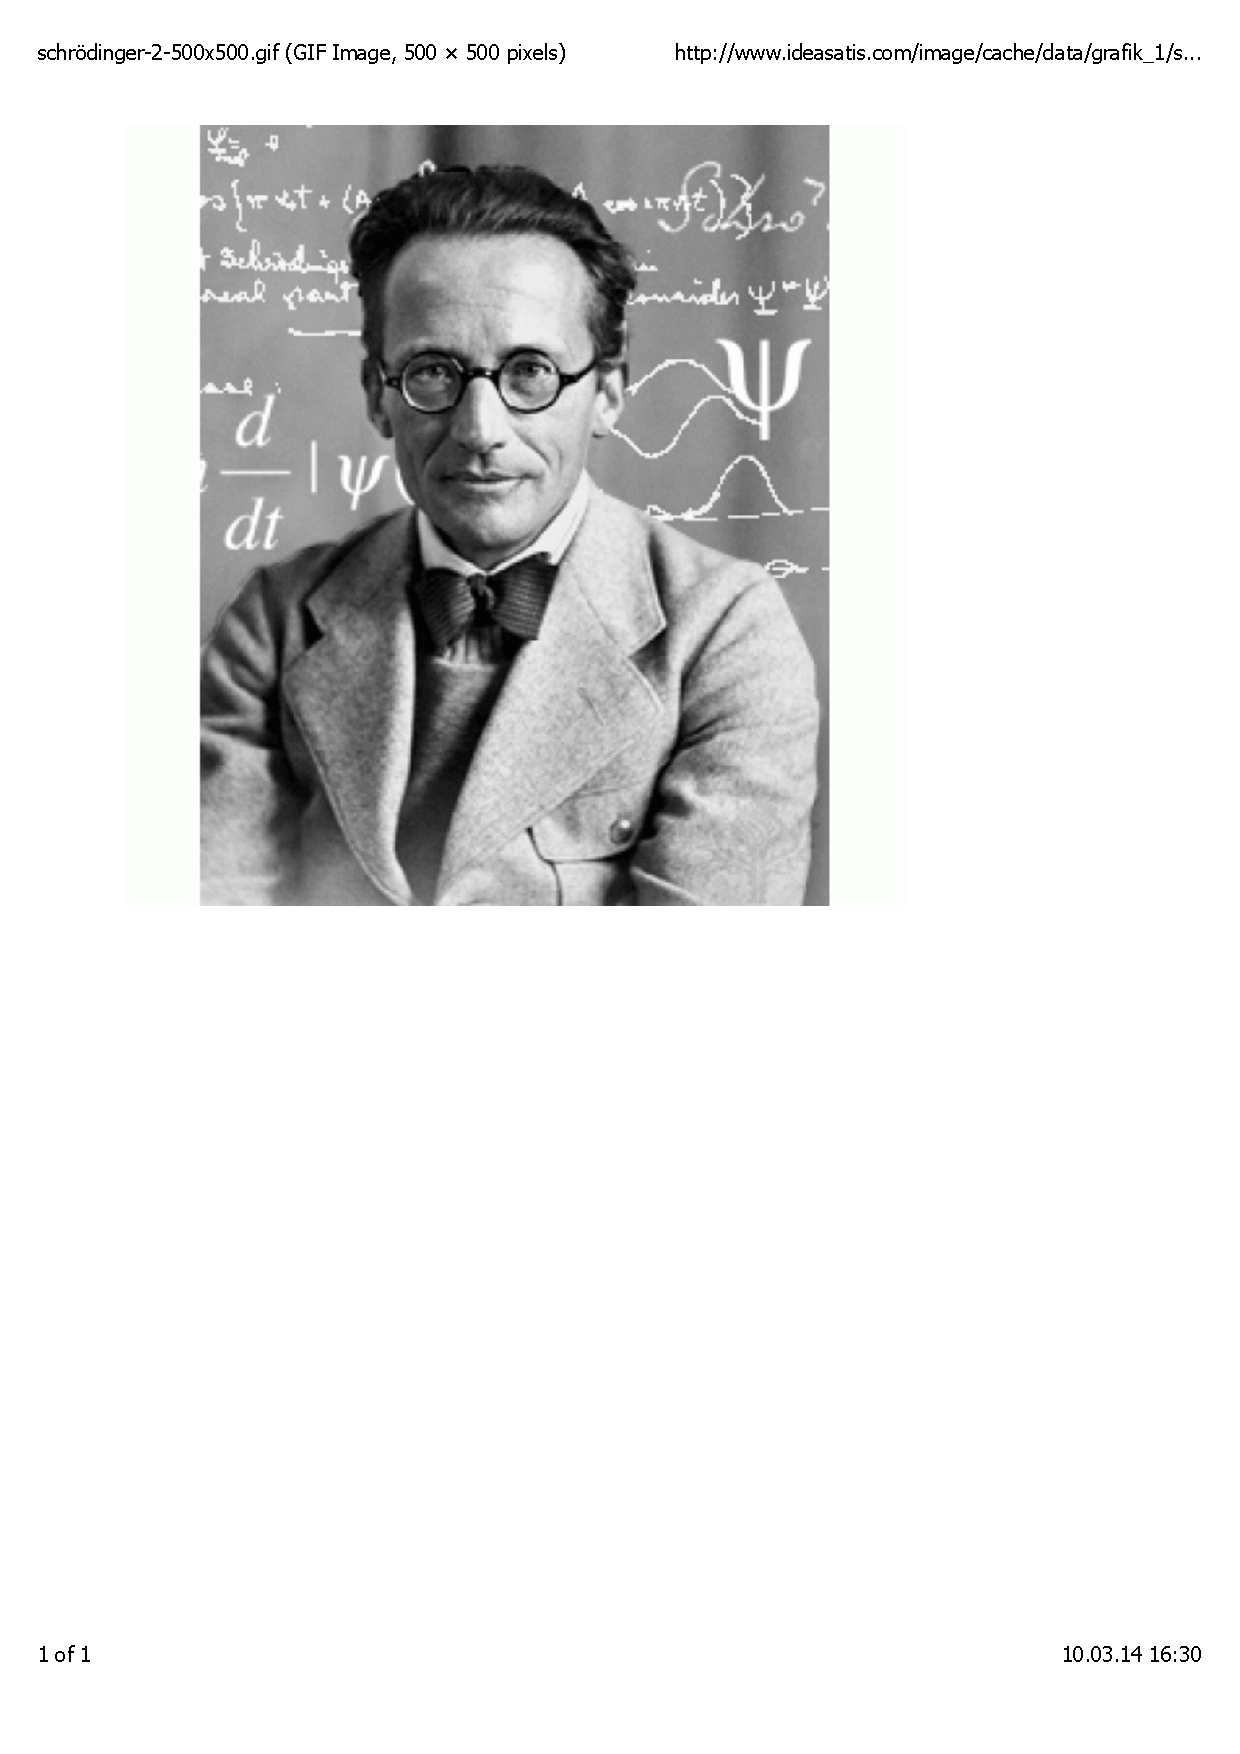
\includegraphics[viewport = 90 405 400 795, clip, scale=0.23]{figures/schrodinger.pdf}
    \end{column}
    \end{columns}
    \ \\
    \ \\
    \begin{equation}
	\nonumber
        h \psi = \left(\frac{\boldsymbol{p}^2}{2m} + V_{Ne} \right) \psi
    \end{equation}
    \ \\
    \begin{equation}
	\nonumber
        g(\boldsymbol{r}_1,\boldsymbol{r}_2) = \frac{1}{r_{12}}
    \end{equation}
\end{frame}

\begin{frame}
    \frametitle{The Dirac equation}
    \begin{columns}
    \begin{column}{.50\textwidth}
	\begin{equation}
	    \nonumber
	    \hat{H} \psi = E \psi
	\end{equation}
	\ \\
	\ \\
	\begin{equation}
	    \nonumber
	    \hat{H} = \sum_i h(\boldsymbol{r}_i) + \frac{1}{2}\sum_{i,j} g(\boldsymbol{r}_i,\boldsymbol{r}_j)
	\end{equation}
    \end{column}
    \begin{column}{.50\textwidth}
	\centering
	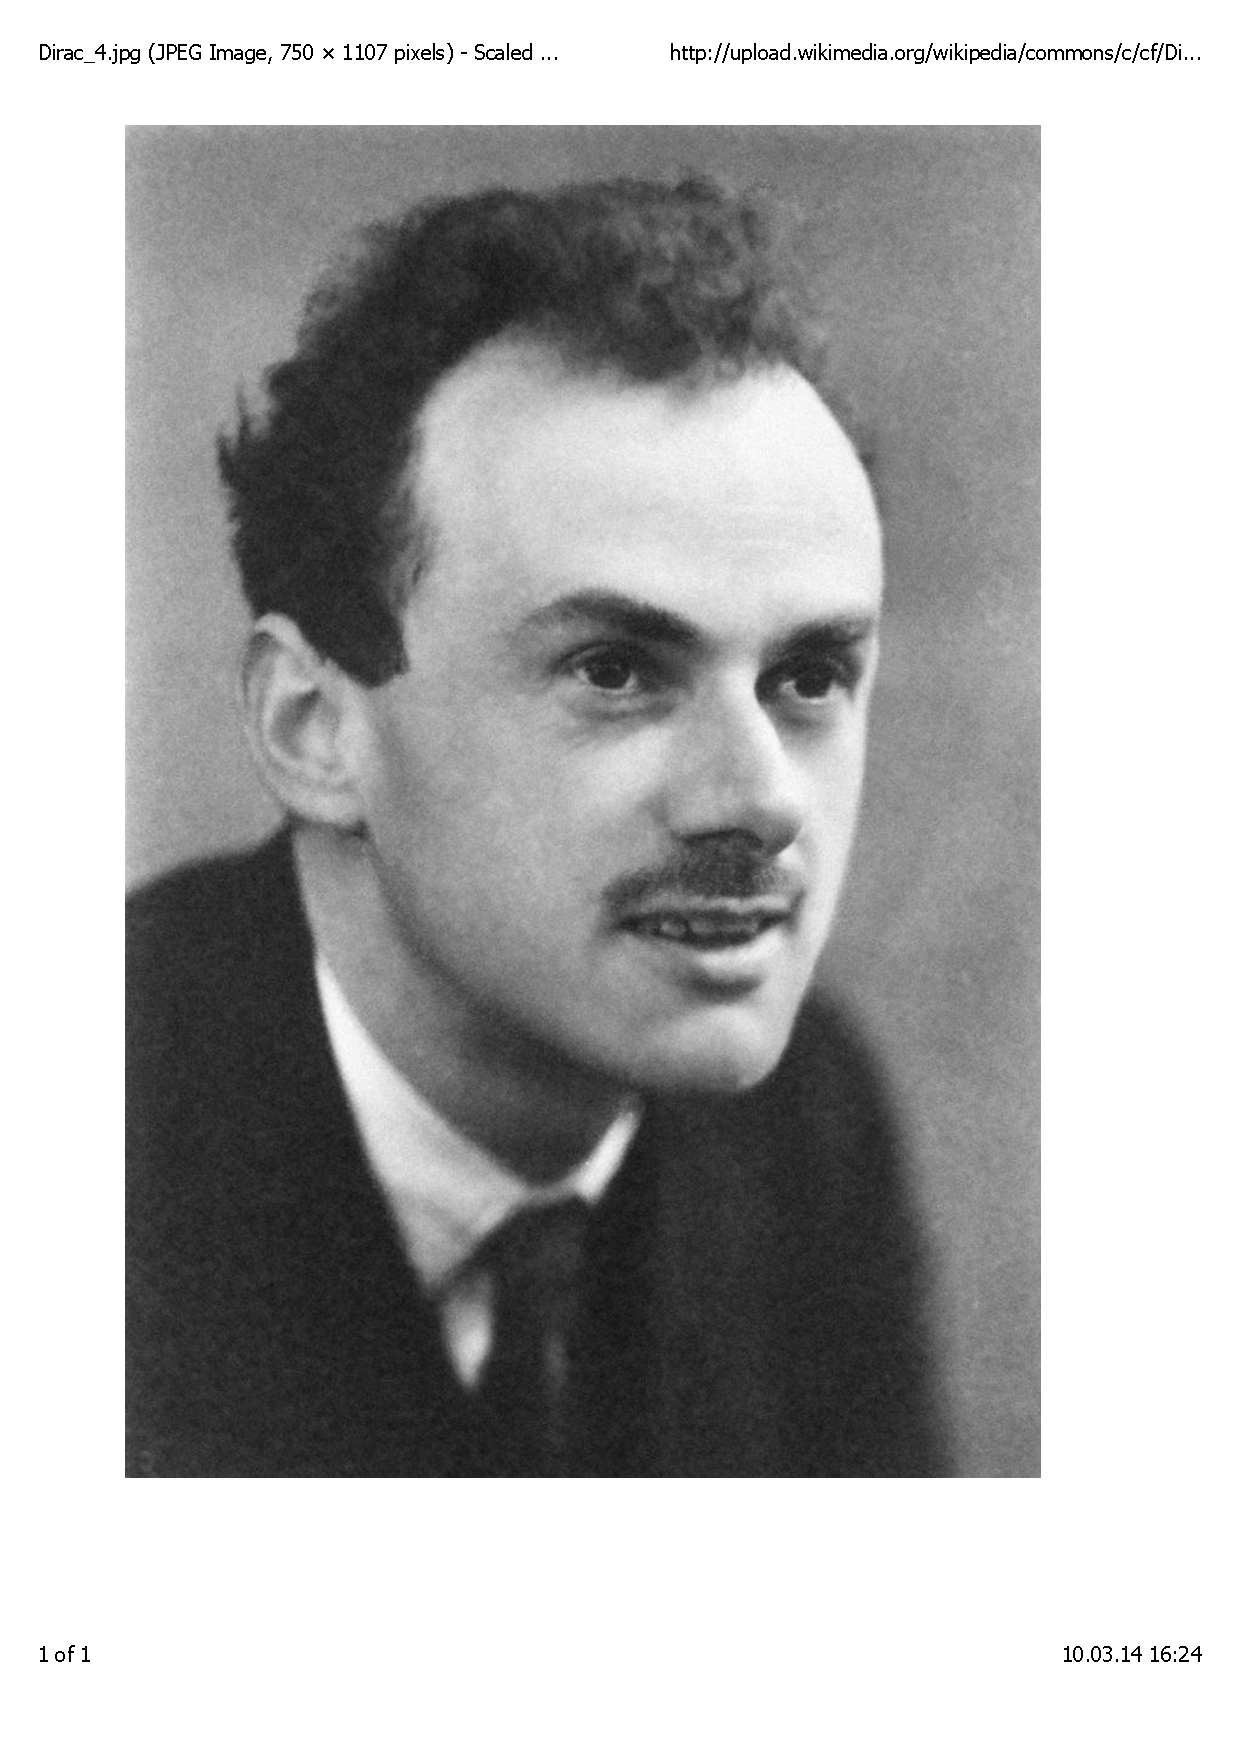
\includegraphics[viewport = 50 200 500 800, clip, scale=0.15]{figures/dirac.pdf}
    \end{column}
    \end{columns}
    \ \\
    \ \\
    \begin{equation}
        \nonumber
        h \psi = 
    	\begin{pmatrix}
	   V_{Ne} I_2 & c\boldsymbol{\sigma}\cdot\boldsymbol{p} \\
	   c\boldsymbol{\sigma}\cdot\boldsymbol{p} & (V_{Ne} - 2mc^2)I_2\\
    	\end{pmatrix}
    	\begin{pmatrix}
	   \psi^L\\
	    \psi^S\\ 
    	\end{pmatrix}
    \end{equation}
    \ \\
    \begin{equation}
        \nonumber
        g(\boldsymbol{r}_i,\boldsymbol{r}_2) = 
        \frac{I_4\cdot I_4}{r_{12}} - \frac{c\boldsymbol{\alpha}_1\cdot c\boldsymbol{\alpha}_2}{c^2r_{12}} -
        \frac{(c\boldsymbol{\alpha}_1\cdot \boldsymbol{r}_{12})(c\boldsymbol{\alpha}_2\cdot \boldsymbol{r}_{12})}{c^2r_{12}^3}
        + \cdots
    \end{equation}
\end{frame}

\begin{frame}
    \frametitle{Relativistic free particle}
    \begin{equation}
	E = \pm \sqrt{\boldsymbol{p}^2c^2+m^2c^4}
    \end{equation}
    Negative energy states
\end{frame}

\begin{frame}
    \frametitle{Relativistic atomic structure}
    Energy expansion\
    Plot of energy levels
\end{frame}

\begin{frame}
    \frametitle{Two-electron interaction}
\end{frame}

\begin{frame}
    \frametitle{Approximate Hamiltonians}
\end{frame}

\begin{frame}
    \frametitle{Scalar relativistic effects}
\end{frame}

\begin{frame}
    \frametitle{Spin-orbit effects}
\end{frame}

\begin{frame}
    \frametitle{Relativistic computational chemistry}
    Three-axis plot
\end{frame}

\begin{frame}
    \frametitle{Relativistic computational chemistry}
    Dirac\\
    ReSpect\\
    Solvent effects
\end{frame}

\begin{frame}
    \frametitle{The periodic table}
    \begin{columns}
    \begin{column}{.40\textwidth}
	\ \\
    \end{column}
    \begin{column}{.60\textwidth}
	\centering
	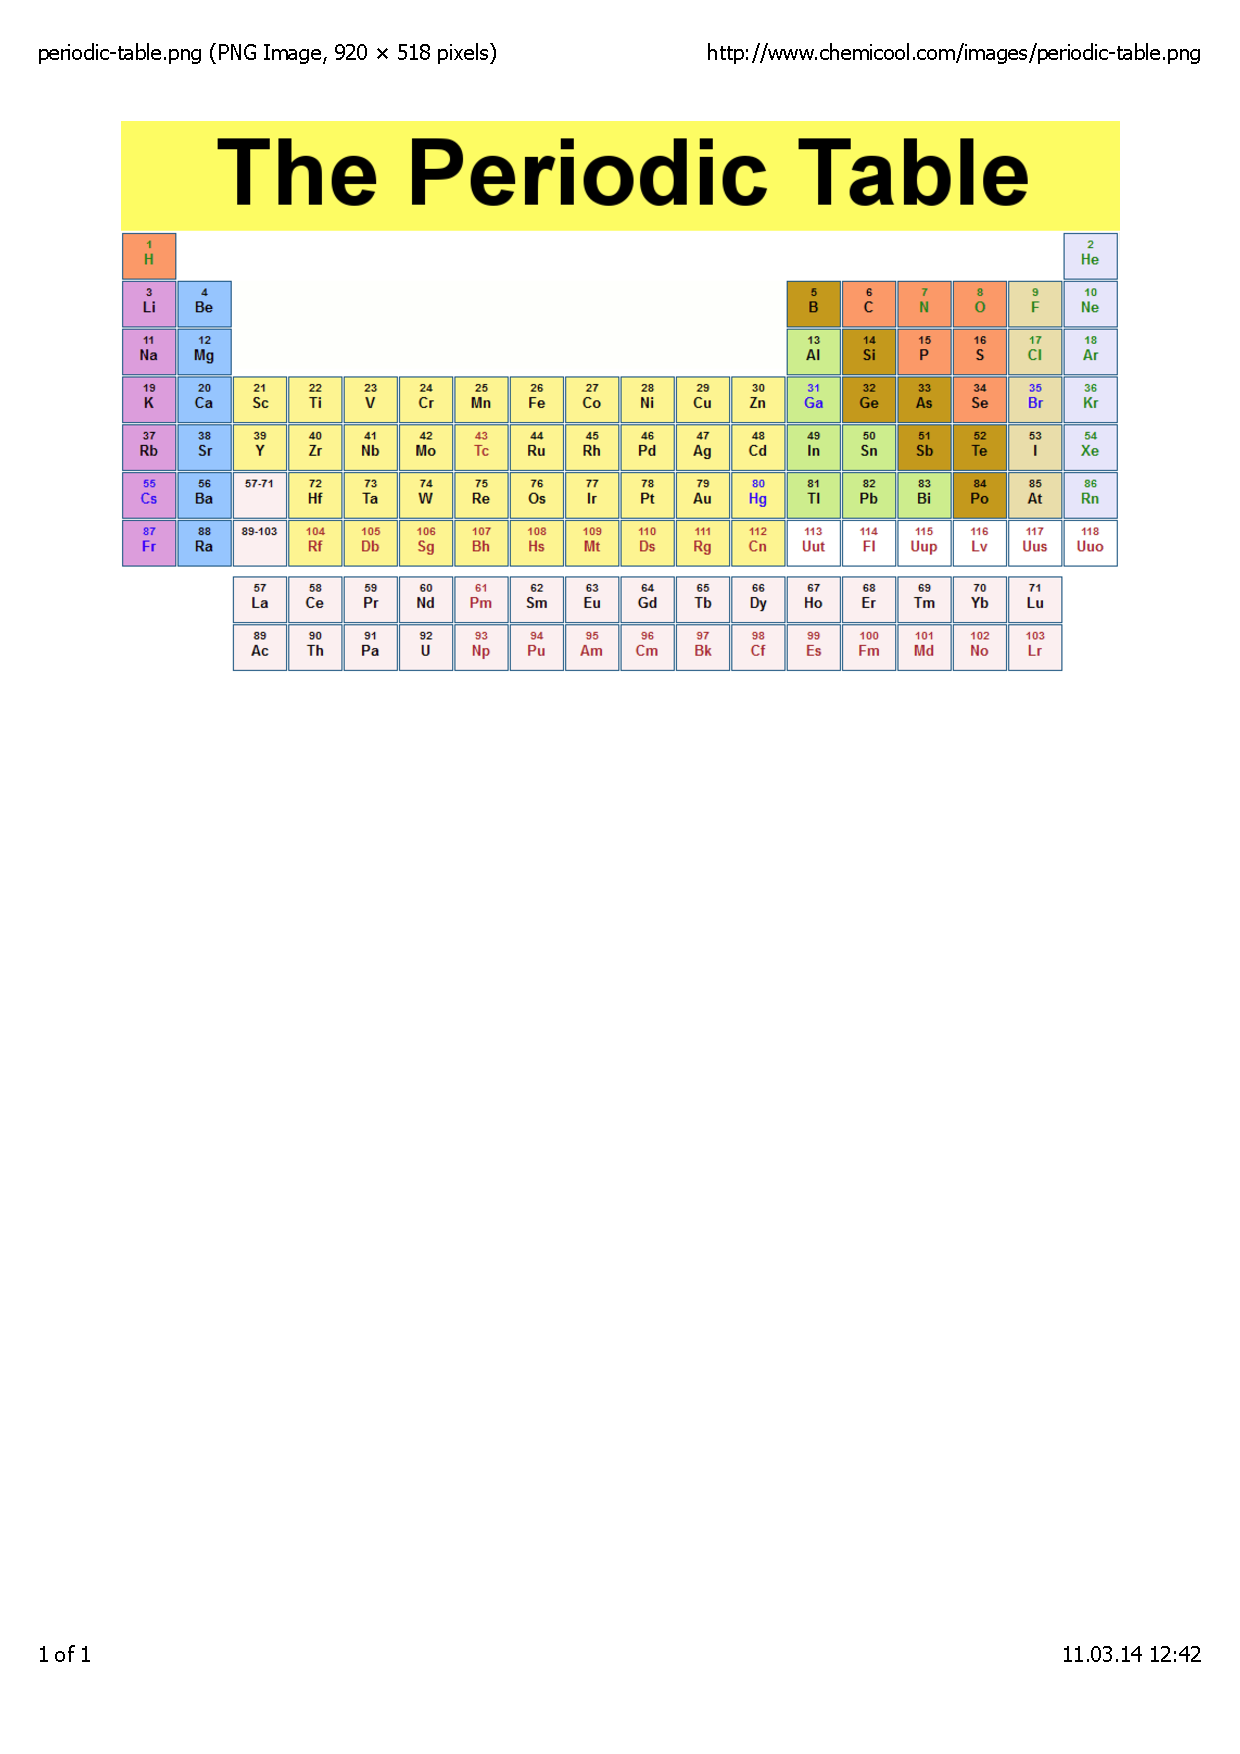
\includegraphics[viewport = 0 500 550 800, clip, scale=0.3]{figures/periodic_table.pdf}
    \end{column}
    \end{columns}
\end{frame}

\begin{frame}
    \frametitle{The color of gold}
    \begin{columns}
    \begin{column}{.50\textwidth}
	\ \\
    \end{column}
    \begin{column}{.50\textwidth}
	\centering
	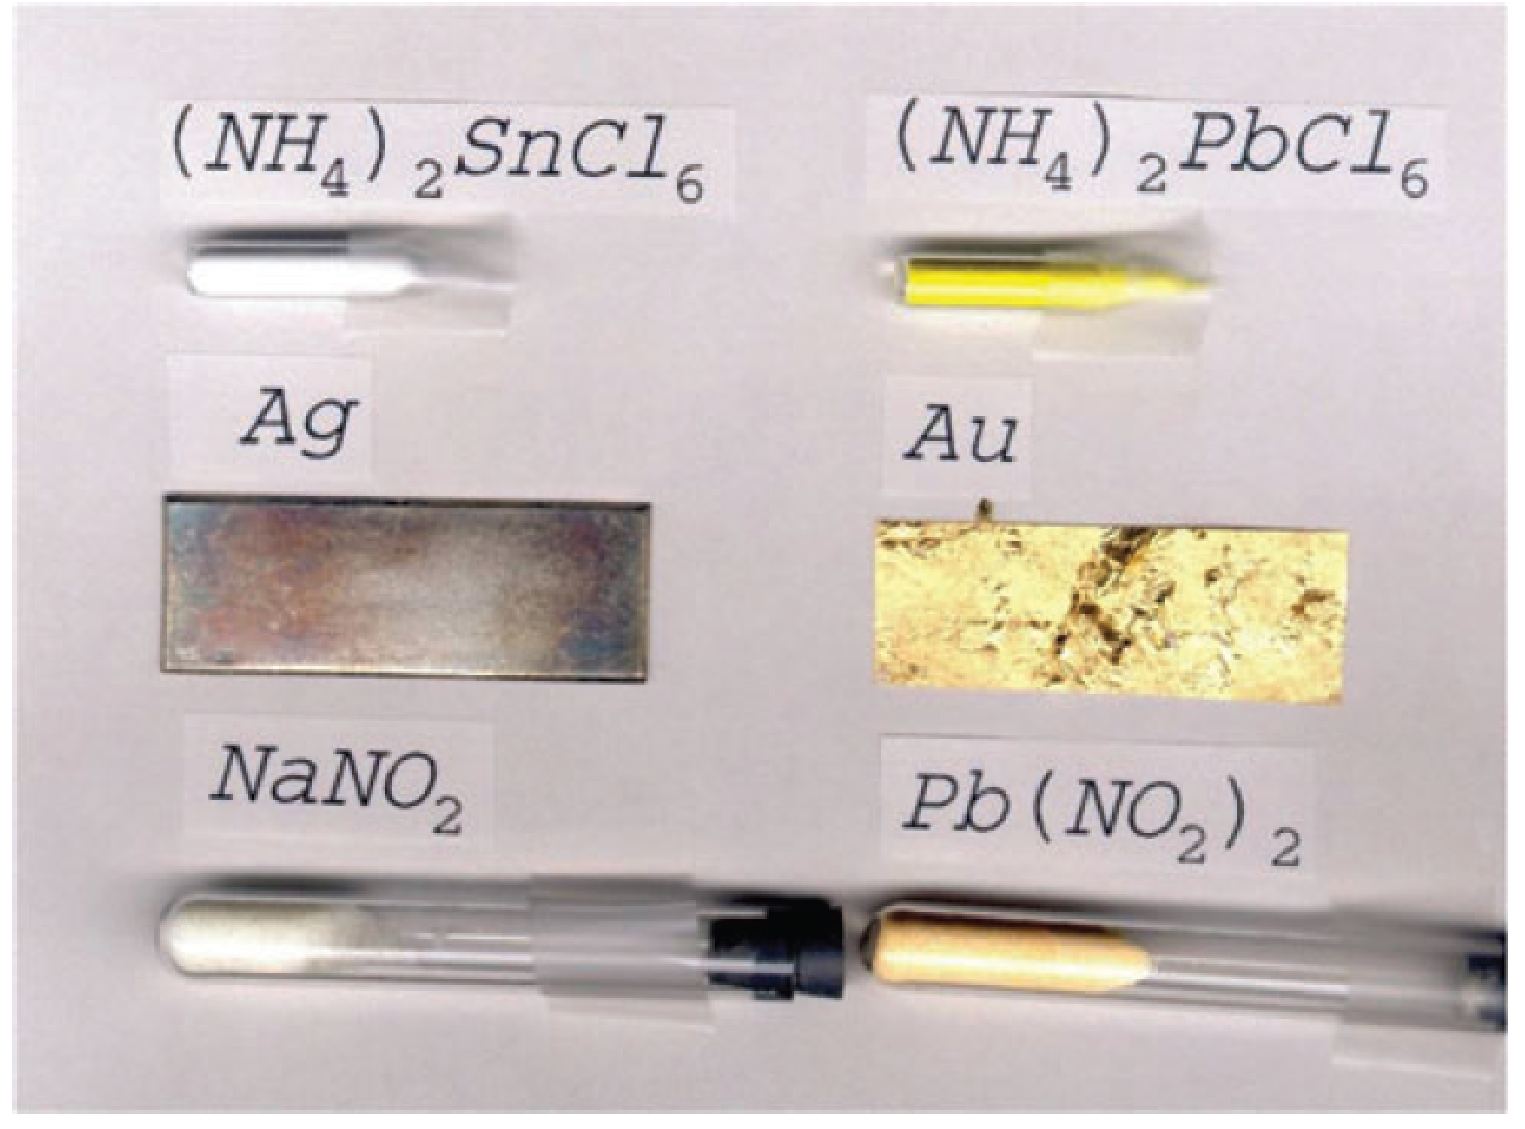
\includegraphics[viewport = 0 0 800 550, clip, scale=0.15]{figures/gold.pdf}
    \end{column}
    \end{columns}
\end{frame}

\begin{frame}
    \frametitle{Lead-acid battery}
    \begin{columns}
    \begin{column}{.50\textwidth}
	\ \\
    \end{column}
    \begin{column}{.50\textwidth}
	\centering
	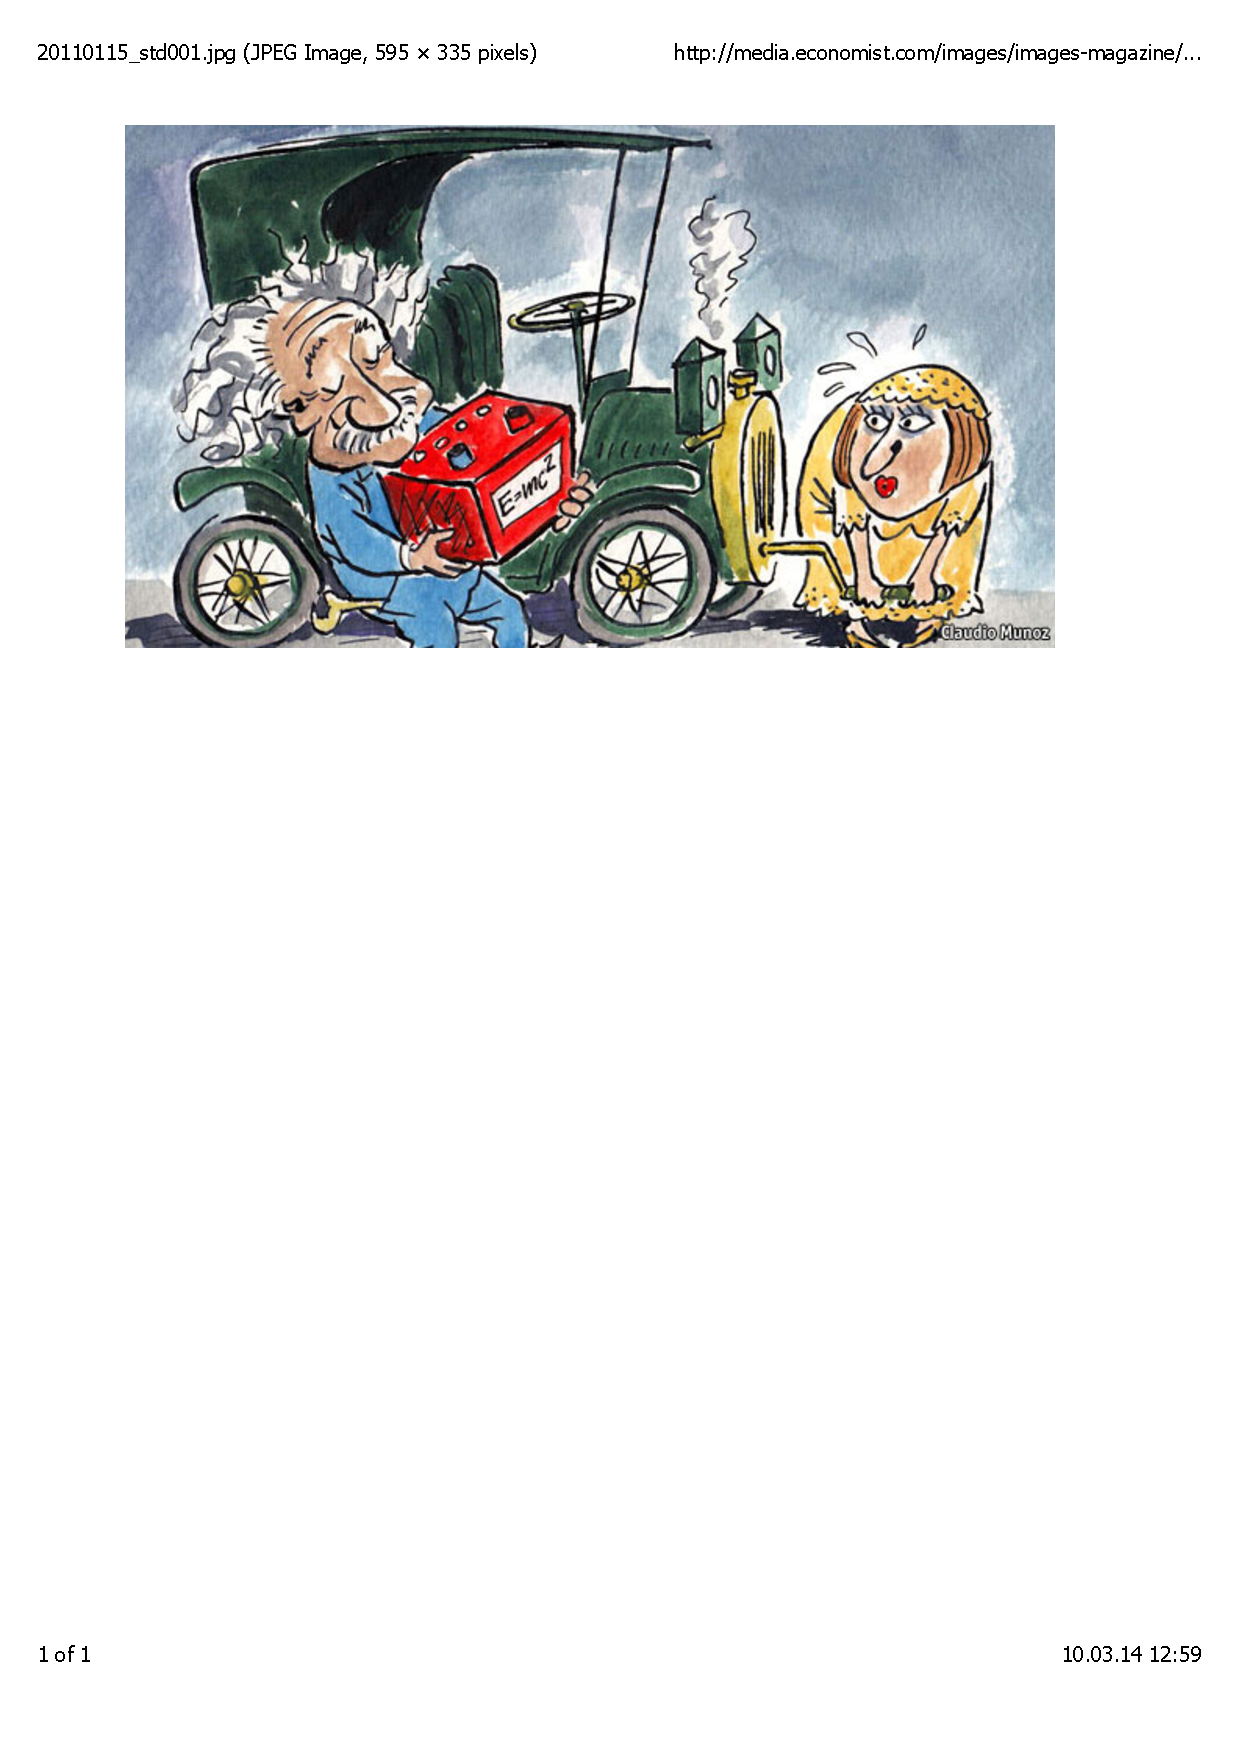
\includegraphics[viewport = 60 530 510 790, clip, scale=0.3]{figures/economist.pdf}
    \end{column}
    \end{columns}
\end{frame}

\begin{frame}
    \frametitle{Aurora borealis}
    \begin{columns}
    \begin{column}{.50\textwidth}
	\ \\
    \end{column}
    \begin{column}{.50\textwidth}
	\centering
	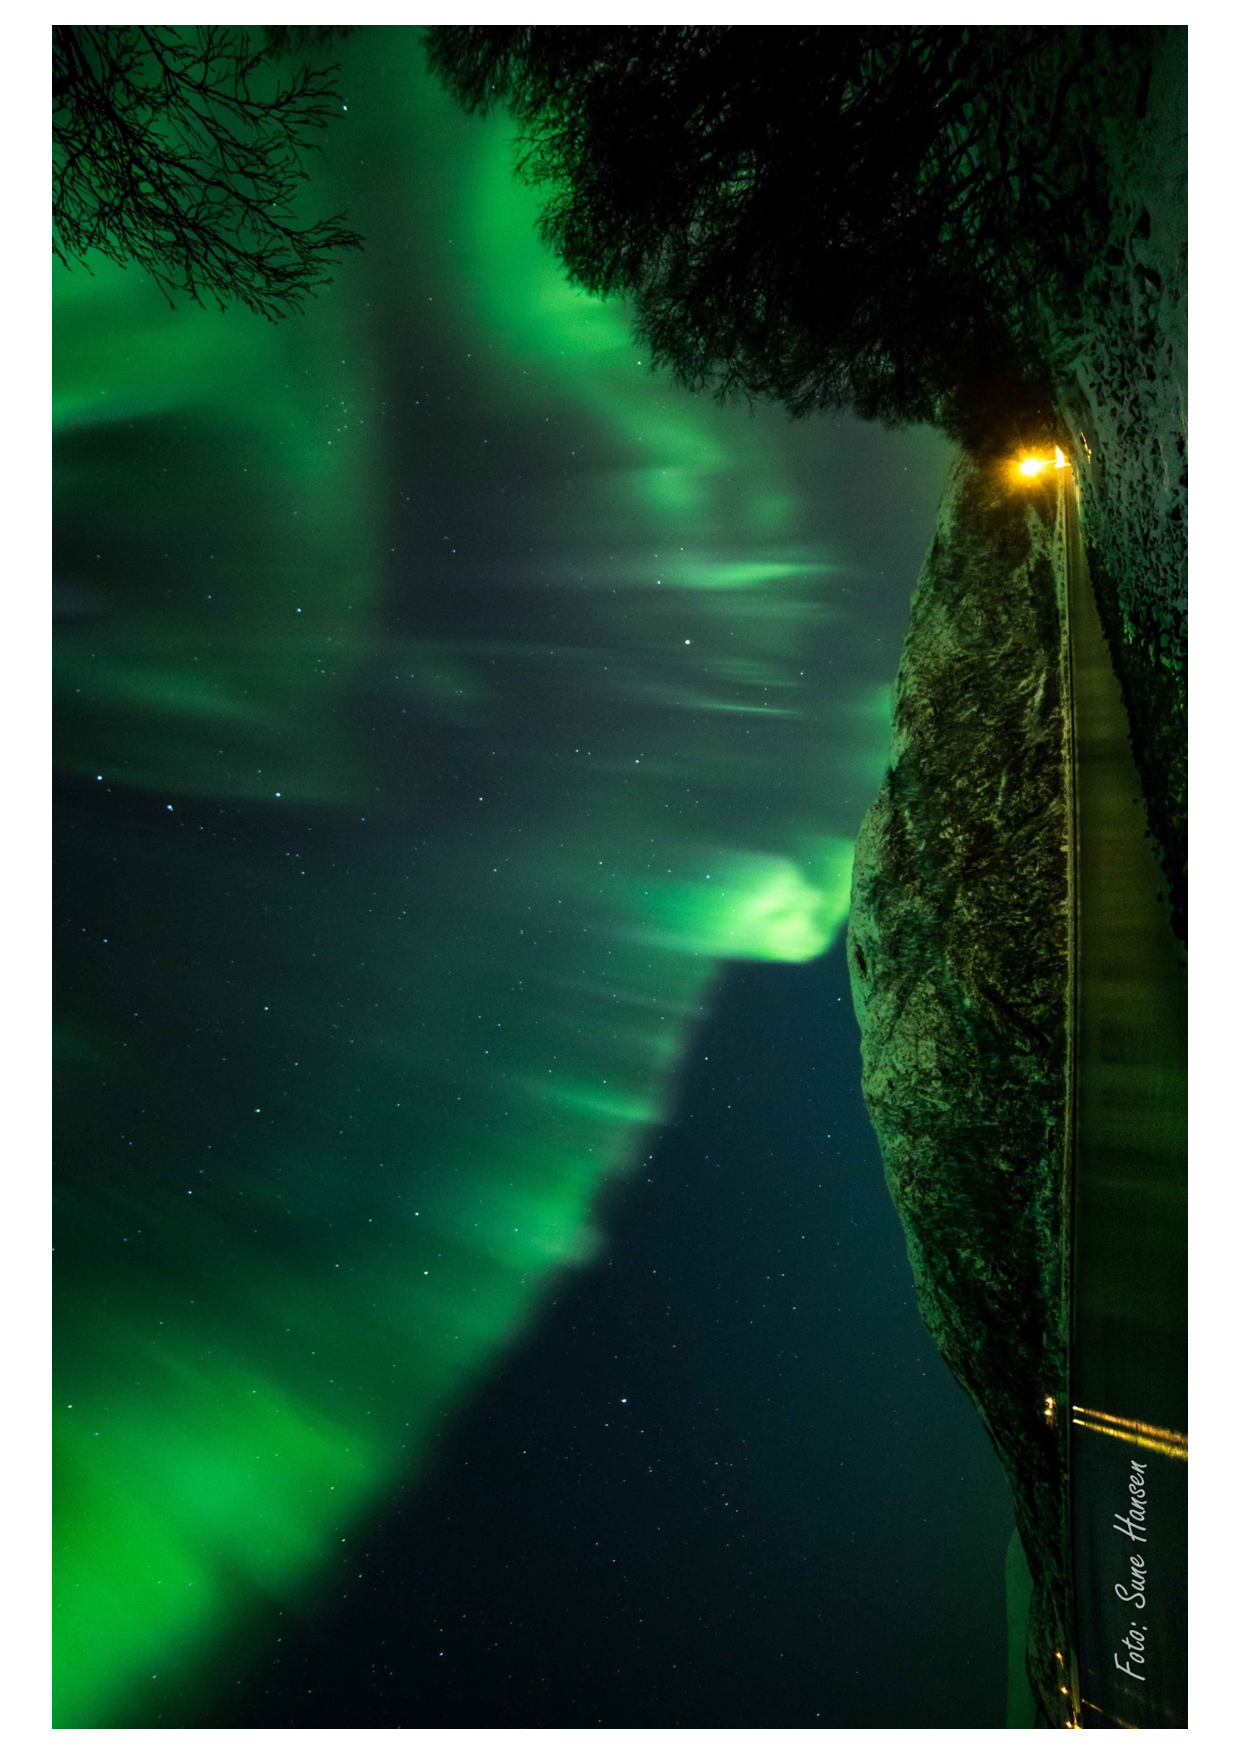
\includegraphics[viewport = 0 0 600 800, clip, scale=0.15, angle = -90]{figures/aurora.pdf}
    \end{column}
    \end{columns}
\end{frame}

\begin{frame}
    \frametitle{Summary}
\end{frame}


\end{document}
